% Reminders:
% - Watch the recordings from Section 3.5 to Section 4.1.3 (included)
% - Complete the third iRAT by Thursday 30th at 13:00
% - Next class on Friday 31st at 11:00.

\subsection*{Question 1}
\textbf{Define the minimum element of a set S (according to Section 3.5).}

The minimum selement $x\in S$ of a set $S$ (with respect to the generalized inequality $\preccurlyeq_K$) is the point that for every $y\in S$, we have $x \preccurlyeq_K y$ ($x \succcurlyeq_K y$). 

\subsection*{Question 2}
\textbf{Define the minimal element of a set S (according to Section 3.5).}

The minimal element $x \in S$ of a set $S$ (with respect to the generalized inequality $\preccurlyeq_K$) is the point that for every $y\in S$, we have $y \preccurlyeq_K x$ ($y \succcurlyeq_K x$) only if $y = x$.

\subsection*{Question 3}
\textbf{Consider a circle and the cone $K = \mathbb{R}^2_+$. Sketch the circle and indicate all minimum and minimal elements in the figure, if any.}

In the figure below, the light shadowed part in the following figure indicates the cone $K = \mathbb{R}^2_+$, and the dark shadowed part represents the circle. 

The minimum element is at the point of the circle's closest distance to the origin, while the minimal element is at the point of the circle's closest distance to the cone.

\begin{center}
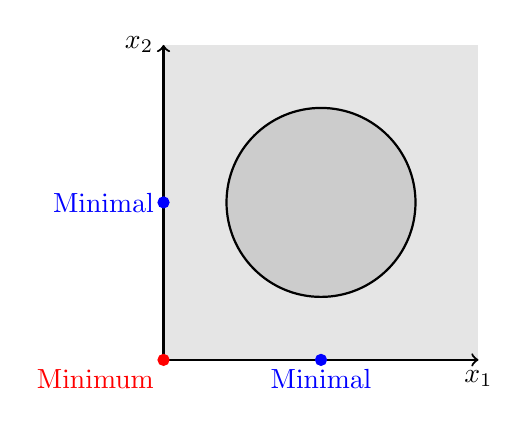
\begin{tikzpicture}
    % K = R^2_+
    \fill[gray!20] (0,0) -- (4,0) -- (4,4) -- (0,4) -- cycle;
    \draw[thick, ->] (0,0) -- (4,0) node[anchor=north] {$x_1$};
    \draw[thick, ->] (0,0) -- (0,4) node[anchor=east] {$x_2$};
    
    % circle
    \fill[gray!40] (2,2) circle (1.2);
    \draw[thick] (2,2) circle (1.2);

    \filldraw[red] (0,0) circle (2pt) node[anchor=north east] {Minimum};
    \filldraw[blue] (0,2) circle (2pt) node[anchor=east] {Minimal};
    \filldraw[blue] (2,0) circle (2pt) node[anchor=north] {Minimal};
\end{tikzpicture}
\hspace{1cm}
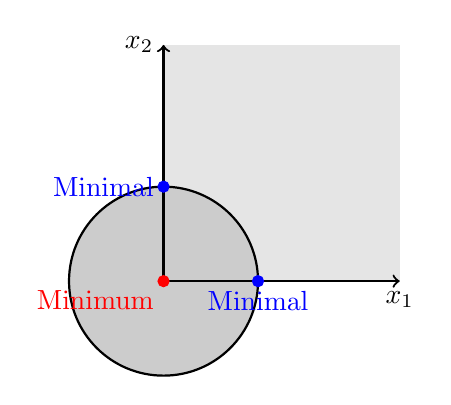
\begin{tikzpicture}
    \fill[gray!20] (0,0) -- (3,0) -- (3,3) -- (0,3) -- cycle;
    \fill[gray!40] (0,0) circle (1.2);
    \draw[thick] (0,0) circle (1.2);
    \draw[thick, ->] (0,0) -- (3,0) node[anchor=north] {$x_1$};
    \draw[thick, ->] (0,0) -- (0,3) node[anchor=east] {$x_2$};

    \filldraw[red] (0,0) circle (2pt) node[anchor=north east] {Minimum};
    \filldraw[blue] (0,1.2) circle (2pt) node[anchor=east] {Minimal};
    \filldraw[blue] (1.2,0) circle (2pt) node[anchor=north] {Minimal};
\end{tikzpicture}
\end{center}

\subsection*{Question 4}
\textbf{Give now the definitions of minimum and minimal elements of S with respect to a cone $K$ using the dual cone $K^*$ (according to Section 3.7).}

$x$ is the minimum element of $S$, with respect to the generalised inequality induced by $K$, if and only if for all $\lambda \succ_{K^*} 0$, $x$ is the unique minimizer of $\lambda^\top z$ over $z \in S$. 

$x$ is a minimal element of $S$, with respect to the generalized inequality induced by $K$, if $\lambda \succ_{K^*} 0$ and $x$ minimizes $\lambda^\top z$ over $z \in S$.

\subsection*{Question 5}
\textbf{Define a convex function in three different ways (1) Jensen's inequality, (2) the first order characterization, (3) the second order characterization.}

1. \textbf{Jensen's inequality:} 

A function $f$ is convex if for all $x$, $y \in \textbf{dom } f$, and $\theta$ with $0 \le \theta \le  1$, we have $ f(\theta x + (1 - \theta)y) \le  \theta f(x) + (1 - \theta)f(y)$. 

2. \textbf{First order characterization:} 

A differentiable function $f$ is convex if and only if $\textbf{dom } f$ is convex and $f(y) \ge f(x) + \nabla f(x)^\top (y-x)$ holds for all $x,y \in \textbf{dom }f$. 

3. \textbf{Second order characterization:} 

A twice differentiable function $f$ is convex if and only if $\textbf{dom }f$ is convex and its Hessian is positive semidefinite, i.e. for all $x \in \textbf{dom }f$ $\nabla^2 f(x) \succcurlyeq 0$. 

\subsection*{Question 6}
\textbf{Explain the meaning and importance of the statement: “the first-order Taylor expansion at a point of a convex function is a global underestimator”.}

We can use the first-order Taylor expansion to do an approximation of a function \( f \) around a point \( x \). For a differentiable function \( f \), the first-order Taylor expansion at point \( x \) is given by $f(y) \approx f(x) + \nabla f(x)^T (y - x) $, where \( \nabla f(x) \) is the gradient of \( f \) at \( x \), and \( (y - x) \) is the vector from \( x \) to \( y \).

This provides a linear function that lies below the graph of \( f \) for all \( y \) in the domain of \( f \). ie.$ f(y) \geq f(x) + \nabla f(x)^T (y - x) \quad \text{for all } y \in \mathbb{R}^n $. 

\textbf{Importance:} 

This inequality shows that from the local information about a convex function (i.e. its value and derivative at a point) we can derive global information (i.e., a global underestimator of it). In this way, we can eventually find the minimum of convex functions by iteratively moving in the direction of the negative gradient. 